\documentclass[]{article}
\usepackage{lmodern}
\usepackage{amssymb,amsmath}
\usepackage{ifxetex,ifluatex}
\usepackage{fixltx2e} % provides \textsubscript
\ifnum 0\ifxetex 1\fi\ifluatex 1\fi=0 % if pdftex
  \usepackage[T1]{fontenc}
  \usepackage[utf8]{inputenc}
\else % if luatex or xelatex
  \ifxetex
    \usepackage{mathspec}
  \else
    \usepackage{fontspec}
  \fi
  \defaultfontfeatures{Ligatures=TeX,Scale=MatchLowercase}
\fi
% use upquote if available, for straight quotes in verbatim environments
\IfFileExists{upquote.sty}{\usepackage{upquote}}{}
% use microtype if available
\IfFileExists{microtype.sty}{%
\usepackage{microtype}
\UseMicrotypeSet[protrusion]{basicmath} % disable protrusion for tt fonts
}{}
\usepackage[margin=1in]{geometry}
\usepackage{hyperref}
\hypersetup{unicode=true,
            pdftitle={Statistical Inference Course Project},
            pdfauthor={A. Johnson},
            pdfborder={0 0 0},
            breaklinks=true}
\urlstyle{same}  % don't use monospace font for urls
\usepackage{color}
\usepackage{fancyvrb}
\newcommand{\VerbBar}{|}
\newcommand{\VERB}{\Verb[commandchars=\\\{\}]}
\DefineVerbatimEnvironment{Highlighting}{Verbatim}{commandchars=\\\{\}}
% Add ',fontsize=\small' for more characters per line
\usepackage{framed}
\definecolor{shadecolor}{RGB}{248,248,248}
\newenvironment{Shaded}{\begin{snugshade}}{\end{snugshade}}
\newcommand{\KeywordTok}[1]{\textcolor[rgb]{0.13,0.29,0.53}{\textbf{#1}}}
\newcommand{\DataTypeTok}[1]{\textcolor[rgb]{0.13,0.29,0.53}{#1}}
\newcommand{\DecValTok}[1]{\textcolor[rgb]{0.00,0.00,0.81}{#1}}
\newcommand{\BaseNTok}[1]{\textcolor[rgb]{0.00,0.00,0.81}{#1}}
\newcommand{\FloatTok}[1]{\textcolor[rgb]{0.00,0.00,0.81}{#1}}
\newcommand{\ConstantTok}[1]{\textcolor[rgb]{0.00,0.00,0.00}{#1}}
\newcommand{\CharTok}[1]{\textcolor[rgb]{0.31,0.60,0.02}{#1}}
\newcommand{\SpecialCharTok}[1]{\textcolor[rgb]{0.00,0.00,0.00}{#1}}
\newcommand{\StringTok}[1]{\textcolor[rgb]{0.31,0.60,0.02}{#1}}
\newcommand{\VerbatimStringTok}[1]{\textcolor[rgb]{0.31,0.60,0.02}{#1}}
\newcommand{\SpecialStringTok}[1]{\textcolor[rgb]{0.31,0.60,0.02}{#1}}
\newcommand{\ImportTok}[1]{#1}
\newcommand{\CommentTok}[1]{\textcolor[rgb]{0.56,0.35,0.01}{\textit{#1}}}
\newcommand{\DocumentationTok}[1]{\textcolor[rgb]{0.56,0.35,0.01}{\textbf{\textit{#1}}}}
\newcommand{\AnnotationTok}[1]{\textcolor[rgb]{0.56,0.35,0.01}{\textbf{\textit{#1}}}}
\newcommand{\CommentVarTok}[1]{\textcolor[rgb]{0.56,0.35,0.01}{\textbf{\textit{#1}}}}
\newcommand{\OtherTok}[1]{\textcolor[rgb]{0.56,0.35,0.01}{#1}}
\newcommand{\FunctionTok}[1]{\textcolor[rgb]{0.00,0.00,0.00}{#1}}
\newcommand{\VariableTok}[1]{\textcolor[rgb]{0.00,0.00,0.00}{#1}}
\newcommand{\ControlFlowTok}[1]{\textcolor[rgb]{0.13,0.29,0.53}{\textbf{#1}}}
\newcommand{\OperatorTok}[1]{\textcolor[rgb]{0.81,0.36,0.00}{\textbf{#1}}}
\newcommand{\BuiltInTok}[1]{#1}
\newcommand{\ExtensionTok}[1]{#1}
\newcommand{\PreprocessorTok}[1]{\textcolor[rgb]{0.56,0.35,0.01}{\textit{#1}}}
\newcommand{\AttributeTok}[1]{\textcolor[rgb]{0.77,0.63,0.00}{#1}}
\newcommand{\RegionMarkerTok}[1]{#1}
\newcommand{\InformationTok}[1]{\textcolor[rgb]{0.56,0.35,0.01}{\textbf{\textit{#1}}}}
\newcommand{\WarningTok}[1]{\textcolor[rgb]{0.56,0.35,0.01}{\textbf{\textit{#1}}}}
\newcommand{\AlertTok}[1]{\textcolor[rgb]{0.94,0.16,0.16}{#1}}
\newcommand{\ErrorTok}[1]{\textcolor[rgb]{0.64,0.00,0.00}{\textbf{#1}}}
\newcommand{\NormalTok}[1]{#1}
\usepackage{graphicx,grffile}
\makeatletter
\def\maxwidth{\ifdim\Gin@nat@width>\linewidth\linewidth\else\Gin@nat@width\fi}
\def\maxheight{\ifdim\Gin@nat@height>\textheight\textheight\else\Gin@nat@height\fi}
\makeatother
% Scale images if necessary, so that they will not overflow the page
% margins by default, and it is still possible to overwrite the defaults
% using explicit options in \includegraphics[width, height, ...]{}
\setkeys{Gin}{width=\maxwidth,height=\maxheight,keepaspectratio}
\IfFileExists{parskip.sty}{%
\usepackage{parskip}
}{% else
\setlength{\parindent}{0pt}
\setlength{\parskip}{6pt plus 2pt minus 1pt}
}
\setlength{\emergencystretch}{3em}  % prevent overfull lines
\providecommand{\tightlist}{%
  \setlength{\itemsep}{0pt}\setlength{\parskip}{0pt}}
\setcounter{secnumdepth}{0}
% Redefines (sub)paragraphs to behave more like sections
\ifx\paragraph\undefined\else
\let\oldparagraph\paragraph
\renewcommand{\paragraph}[1]{\oldparagraph{#1}\mbox{}}
\fi
\ifx\subparagraph\undefined\else
\let\oldsubparagraph\subparagraph
\renewcommand{\subparagraph}[1]{\oldsubparagraph{#1}\mbox{}}
\fi

%%% Use protect on footnotes to avoid problems with footnotes in titles
\let\rmarkdownfootnote\footnote%
\def\footnote{\protect\rmarkdownfootnote}

%%% Change title format to be more compact
\usepackage{titling}

% Create subtitle command for use in maketitle
\providecommand{\subtitle}[1]{
  \posttitle{
    \begin{center}\large#1\end{center}
    }
}

\setlength{\droptitle}{-2em}

  \title{Statistical Inference Course Project}
    \pretitle{\vspace{\droptitle}\centering\huge}
  \posttitle{\par}
    \author{A. Johnson}
    \preauthor{\centering\large\emph}
  \postauthor{\par}
      \predate{\centering\large\emph}
  \postdate{\par}
    \date{10 August 2019}


\begin{document}
\maketitle

\subsection{Synopsis}\label{synopsis}

The project consists of two parts:

\begin{verbatim}
    - A simulation exercise
    
    - Basic inferential data analysis
\end{verbatim}

Given the nature of the series, I used knitr to create the reports and
convert to a pdf. The pdf report was limited to be no more than 3 pages
with 3 pages of supporting appendix material if needed (code, figures,
etc.).

\subsection{Review Criteria}\label{review-criteria}

The project required us to answer the following questions:

\begin{verbatim}
    - What were the basic features of the data? 
    
    - Where was the distribution centered and how did it compare to the theoretical center of the distribution?
    
    - What was the sample variance and how did it compare to the theoretical variance of the distribution?
    
    - When is it appropriate to present confidence intervals and/or tests? 
    
    - What assumptions are needed for additional context in the conclusions? 
\end{verbatim}

\subsection{Part 1: Simulation Exercise
Instructions}\label{part-1-simulation-exercise-instructions}

In this project I investigated the exponential distribution in R and
compared it with the Central Limit Theorem. The exponential distribution
can be simulated in R with rexp(n, lambda) where lambda is the rate
parameter. The mean of exponential distribution is 1/lambda and the
standard deviation is also 1/lambda. I've set lambda = 0.2 for all of
the simulations. I also investigated the distribution of averages of 40
exponentials and completed 1,000 simulations. Note - Before starting, I
installed and loaded the following packages in R: R.utils, rmarkdown,
knitr, tidyverse, ggplot2, and UsingR.

I illustrated via simulation and associated explanatory text the
properties of the distribution of the mean of 40 exponentials:

\begin{itemize}
\tightlist
\item
  Displayed the sample mean and compared it to the theoretical mean of
  the distribution.
\item
  Demonstrated how variable the sample is (via variance) and compared it
  to the theoretical variance of the distribution.
\item
  Displayed that the distribution is approximately normal.
\end{itemize}

\begin{Shaded}
\begin{Highlighting}[]
        \CommentTok{# Using pre-defined parameters}
\NormalTok{        lambda =}\StringTok{ }\FloatTok{0.2}
\NormalTok{        n =}\StringTok{ }\DecValTok{40}
\NormalTok{        sims =}\StringTok{ }\DecValTok{1}\OperatorTok{:}\DecValTok{1000}
        \KeywordTok{set.seed}\NormalTok{(}\DecValTok{1234}\NormalTok{)}

        
        \CommentTok{# From directions: }
        \CommentTok{# The exponential distribution can be simulated in R with rexp(n, lambda) }
        \CommentTok{# where lambda is the rate parameter. }
        \CommentTok{# The mean of exponential distribution is 1/lambda and the standard deviation is also 1/lambda.}
        
        \CommentTok{# Simulate the population:}
\NormalTok{        pop =}\StringTok{ }\KeywordTok{data.frame}\NormalTok{(}\DataTypeTok{x=}\KeywordTok{sapply}\NormalTok{(sims, }\ControlFlowTok{function}\NormalTok{(x) \{}
                \KeywordTok{mean}\NormalTok{(}\KeywordTok{rexp}\NormalTok{(n, lambda))}
\NormalTok{        \}))}
\end{Highlighting}
\end{Shaded}

\begin{Shaded}
\begin{Highlighting}[]
        \CommentTok{# Plot the histogram}
        \KeywordTok{ggplot}\NormalTok{(pop, }\KeywordTok{aes}\NormalTok{(}\DataTypeTok{x=}\NormalTok{x)) }\OperatorTok{+}
\StringTok{                }\KeywordTok{geom_histogram}\NormalTok{(}\KeywordTok{aes}\NormalTok{(}\DataTypeTok{y=}\NormalTok{..count.., }\DataTypeTok{fill=}\NormalTok{..count..), }
                               \DataTypeTok{color =} \StringTok{"black"}\NormalTok{) }\OperatorTok{+}\StringTok{ }
\StringTok{                }\KeywordTok{labs}\NormalTok{(}\DataTypeTok{title=}\StringTok{"Distribution of Means of 40 Exponentials ~ 1000 Simulations"}\NormalTok{, }
                     \DataTypeTok{y=}\StringTok{"Frequency Count"}\NormalTok{, }\DataTypeTok{x=}\StringTok{"Mean"}\NormalTok{)}
\end{Highlighting}
\end{Shaded}

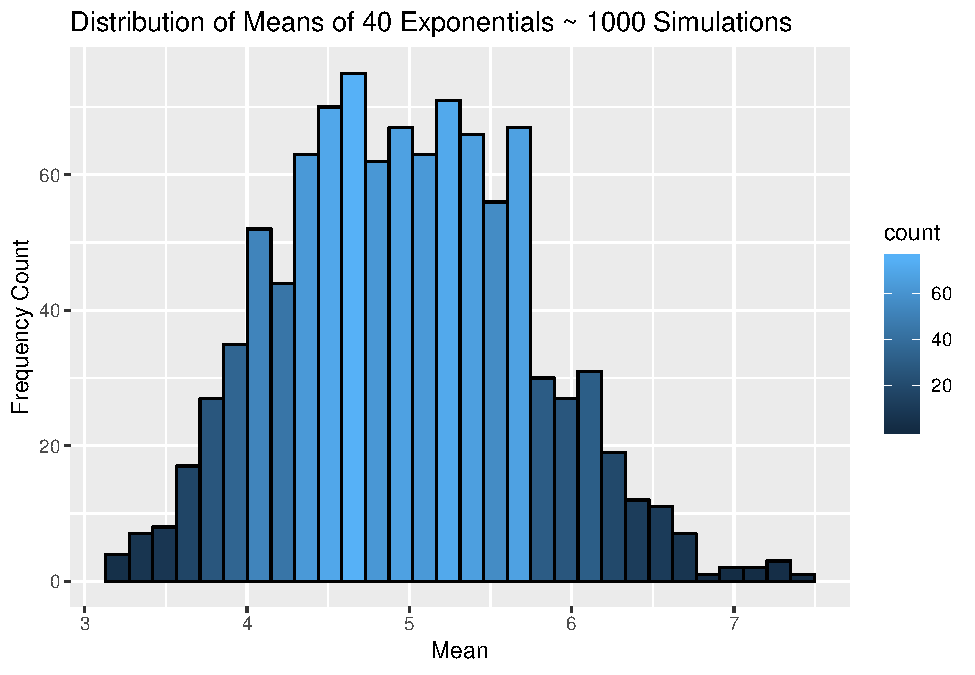
\includegraphics{figures/fig-EDAhisto-1.pdf}

I used the pre-defined parameters and set the seed at 1234. By sampling
without replacement, the plot visualizes that the mean is around 5. The
distribution in the plot seems to be approximating a normal
distribution, however, there is uneven distribution in the tails.

\begin{Shaded}
\begin{Highlighting}[]
\CommentTok{# Show the sample mean and compare it to the theoretical mean of the distribution.}
\NormalTok{        sample.mean =}\StringTok{ }\KeywordTok{round}\NormalTok{(}\KeywordTok{mean}\NormalTok{(pop}\OperatorTok{$}\NormalTok{x), }\DecValTok{2}\NormalTok{)}
\NormalTok{        theo.mean =}\StringTok{ }\KeywordTok{round}\NormalTok{(}\DecValTok{1}\OperatorTok{/}\NormalTok{lambda, }\DecValTok{2}\NormalTok{)}
        \KeywordTok{cbind}\NormalTok{(sample.mean, theo.mean)}
\end{Highlighting}
\end{Shaded}

\begin{verbatim}
##      sample.mean theo.mean
## [1,]        4.97         5
\end{verbatim}

The sample mean (4.97) approximates the theoretical mean (5).

\begin{Shaded}
\begin{Highlighting}[]
\CommentTok{# Check the 95% confidence interval for the sample mean}
        \KeywordTok{t.test}\NormalTok{(pop}\OperatorTok{$}\NormalTok{x)}
\end{Highlighting}
\end{Shaded}

\begin{verbatim}
## 
##  One Sample t-test
## 
## data:  pop$x
## t = 208.23, df = 999, p-value < 0.00000000000000022
## alternative hypothesis: true mean is not equal to 0
## 95 percent confidence interval:
##  4.927362 5.021116
## sample estimates:
## mean of x 
##  4.974239
\end{verbatim}

\begin{Shaded}
\begin{Highlighting}[]
\NormalTok{        ci =}\StringTok{ }\KeywordTok{t.test}\NormalTok{(pop}\OperatorTok{$}\NormalTok{x)}\OperatorTok{$}\NormalTok{conf}
\NormalTok{        lowerci =}\StringTok{ }\KeywordTok{round}\NormalTok{(ci[}\DecValTok{1}\NormalTok{], }\DecValTok{2}\NormalTok{)}
\NormalTok{        upperci =}\StringTok{ }\KeywordTok{round}\NormalTok{(ci[}\DecValTok{2}\NormalTok{], }\DecValTok{2}\NormalTok{)}
\end{Highlighting}
\end{Shaded}

The 95\% CI for the sample mean (4.93, 5.02) includes the theoretical
mean (5).

\begin{Shaded}
\begin{Highlighting}[]
\CommentTok{# Show how variable the sample is (via variance) and compare it to the theoretical variance of the }
\CommentTok{# distribution.}
        
\NormalTok{        sample.var =}\StringTok{ }\KeywordTok{round}\NormalTok{(}\KeywordTok{var}\NormalTok{(pop}\OperatorTok{$}\NormalTok{x), }\DecValTok{2}\NormalTok{)}
\NormalTok{        theo.var =}\StringTok{ }\KeywordTok{round}\NormalTok{(((}\DecValTok{1}\OperatorTok{/}\NormalTok{lambda)}\OperatorTok{^}\DecValTok{2}\NormalTok{)}\OperatorTok{/}\NormalTok{n, }\DecValTok{2}\NormalTok{)}
        \KeywordTok{cbind}\NormalTok{(sample.var, theo.var)}
\end{Highlighting}
\end{Shaded}

\begin{verbatim}
##      sample.var theo.var
## [1,]       0.57     0.62
\end{verbatim}

The sample variance (0.57) and the theoretical variance (0.62) are
pretty close to each other.

\begin{Shaded}
\begin{Highlighting}[]
\CommentTok{# Show that the distribution is approximately normal.}
        
         \CommentTok{# Plot the sample mean and var vs. theoretical mean and var:}
        \CommentTok{#We need to plot the density rather than the count because we are }
        \CommentTok{#also plotting the geom_vlines. These would be flattened }
        \CommentTok{#on the bottom of the y-axis (<1) if the y-axis was count.}
        \KeywordTok{ggplot}\NormalTok{(pop, }\KeywordTok{aes}\NormalTok{(}\DataTypeTok{x=}\NormalTok{x)) }\OperatorTok{+}
\StringTok{                }\KeywordTok{geom_histogram}\NormalTok{(}\KeywordTok{aes}\NormalTok{(}\DataTypeTok{y=}\NormalTok{..density.., }\DataTypeTok{fill =}\NormalTok{ ..density..), }
                               \DataTypeTok{color =} \StringTok{"black"}\NormalTok{) }\OperatorTok{+}
\StringTok{                }\KeywordTok{labs}\NormalTok{(}\DataTypeTok{title=}\StringTok{"Sample Distribution of Means of 40 Exponentials ~ 1000 Simulations Against Theoretical Distribution of Means"}\NormalTok{, }
                     \DataTypeTok{y =} \StringTok{"Density"}\NormalTok{, }
                     \DataTypeTok{x =} \StringTok{"Mean"}\NormalTok{, }
                     \DataTypeTok{caption =} \StringTok{"Black = Sample Mean, Red = Theoretical Mean"}\NormalTok{) }\OperatorTok{+}
\StringTok{                }\KeywordTok{geom_density}\NormalTok{(}\DataTypeTok{color =} \StringTok{"black"}\NormalTok{) }\OperatorTok{+}
\StringTok{                }\KeywordTok{geom_vline}\NormalTok{(}\DataTypeTok{xintercept =}\NormalTok{ sample.mean, }\DataTypeTok{color =} \StringTok{"black"}\NormalTok{, }\DataTypeTok{linetype =} \StringTok{"dashed"}\NormalTok{, }\DataTypeTok{show.legend =} \OtherTok{TRUE}\NormalTok{) }\OperatorTok{+}
\StringTok{                }\KeywordTok{stat_function}\NormalTok{(}\DataTypeTok{fun =}\NormalTok{ dnorm, }\DataTypeTok{args =} \KeywordTok{list}\NormalTok{(}\DataTypeTok{mean =} \DecValTok{1}\OperatorTok{/}\NormalTok{lambda, }\DataTypeTok{sd =} \KeywordTok{sqrt}\NormalTok{(theo.var)), }
                              \DataTypeTok{color =} \StringTok{"red"}\NormalTok{) }\OperatorTok{+}
\StringTok{                }\KeywordTok{geom_vline}\NormalTok{(}\DataTypeTok{xintercept =}\NormalTok{ theo.mean, }\DataTypeTok{color =} \StringTok{"red"}\NormalTok{, }\DataTypeTok{linetype =} \StringTok{"dashed"}\NormalTok{, }\DataTypeTok{show.legend =} \OtherTok{TRUE}\NormalTok{)}
\end{Highlighting}
\end{Shaded}

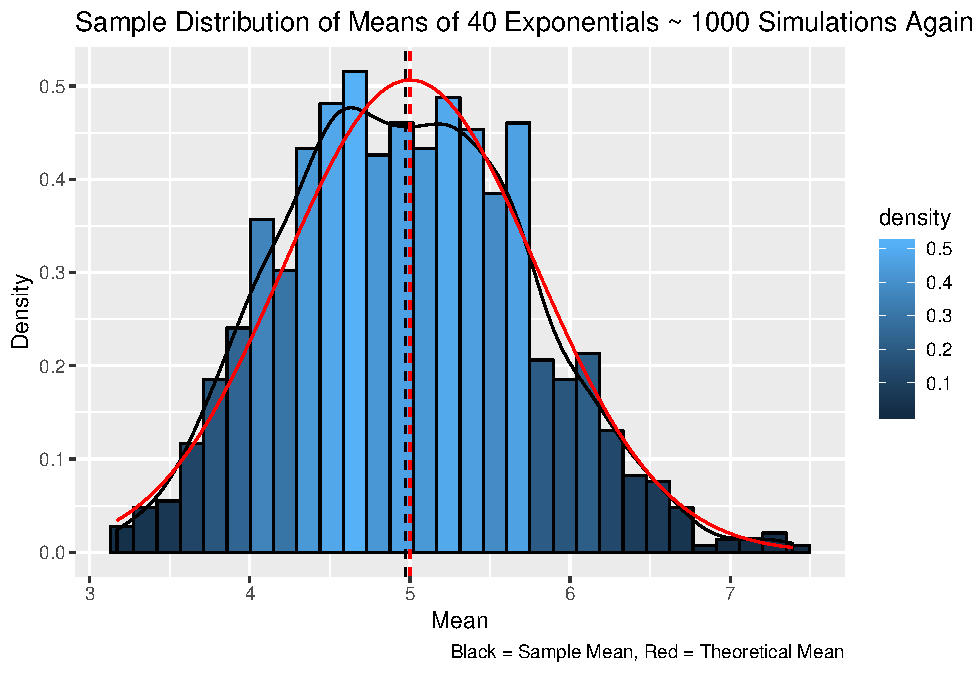
\includegraphics{figures/fig-dist-1.pdf}

Evaluating the figure, the distribution of the sample mean for 40
exponentials simulated 1000 times approximates the theoretical mean for
a normal distribution. You can see this by comparing the shape of the
black line compared to the shape of the red line. The mean from the
sample mean distribution (black vertical dashed line) is slightly lower
than the mean from the theoretical mean distribution (red vertical
dashed line).

\subsection{Part 2: Basic Inferential Data Analysis
Instructions}\label{part-2-basic-inferential-data-analysis-instructions}

In the second portion of the project, I analyzed the ToothGrowth data in
the R datasets package.

\begin{Shaded}
\begin{Highlighting}[]
        \KeywordTok{data}\NormalTok{(ToothGrowth)}
\end{Highlighting}
\end{Shaded}

First, I wanted to see a basic summary of the data:

\begin{Shaded}
\begin{Highlighting}[]
        \CommentTok{# Provide a basic summary of the data.}
        \KeywordTok{str}\NormalTok{(ToothGrowth)}
\end{Highlighting}
\end{Shaded}

\begin{verbatim}
## 'data.frame':    60 obs. of  3 variables:
##  $ len : num  4.2 11.5 7.3 5.8 6.4 10 11.2 11.2 5.2 7 ...
##  $ supp: Factor w/ 2 levels "OJ","VC": 2 2 2 2 2 2 2 2 2 2 ...
##  $ dose: num  0.5 0.5 0.5 0.5 0.5 0.5 0.5 0.5 0.5 0.5 ...
\end{verbatim}

\begin{Shaded}
\begin{Highlighting}[]
        \KeywordTok{summary}\NormalTok{(ToothGrowth)}
\end{Highlighting}
\end{Shaded}

\begin{verbatim}
##       len        supp         dose      
##  Min.   : 4.20   OJ:30   Min.   :0.500  
##  1st Qu.:13.07   VC:30   1st Qu.:0.500  
##  Median :19.25           Median :1.000  
##  Mean   :18.81           Mean   :1.167  
##  3rd Qu.:25.27           3rd Qu.:2.000  
##  Max.   :33.90           Max.   :2.000
\end{verbatim}

\begin{Shaded}
\begin{Highlighting}[]
        \KeywordTok{summary}\NormalTok{(ToothGrowth}\OperatorTok{$}\NormalTok{len }\OperatorTok{~}\StringTok{ }\NormalTok{ToothGrowth}\OperatorTok{$}\NormalTok{supp)}
\end{Highlighting}
\end{Shaded}

\begin{verbatim}
## ToothGrowth$len     N= 60 
## 
## +----------------+--+--+---------------+
## |                |  |N |ToothGrowth$len|
## +----------------+--+--+---------------+
## |ToothGrowth$supp|OJ|30|20.66333       |
## |                |VC|30|16.96333       |
## +----------------+--+--+---------------+
## |Overall         |  |60|18.81333       |
## +----------------+--+--+---------------+
\end{verbatim}

\begin{Shaded}
\begin{Highlighting}[]
        \KeywordTok{summary}\NormalTok{(ToothGrowth}\OperatorTok{$}\NormalTok{len }\OperatorTok{~}\StringTok{ }\NormalTok{ToothGrowth}\OperatorTok{$}\NormalTok{dose)}
\end{Highlighting}
\end{Shaded}

\begin{verbatim}
## ToothGrowth$len     N= 60 
## 
## +----------------+---+--+---------------+
## |                |   |N |ToothGrowth$len|
## +----------------+---+--+---------------+
## |ToothGrowth$dose|0.5|20|10.60500       |
## |                |1  |20|19.73500       |
## |                |2  |20|26.10000       |
## +----------------+---+--+---------------+
## |Overall         |   |60|18.81333       |
## +----------------+---+--+---------------+
\end{verbatim}

This dataframe includes n=60 observations and contains three variables:
len, supp, and dose. The supp variable is two-levels, ``OJ'' and ``VC'',
each containing n=30 observations. The len variable is numeric with a
range of 4.20-33.90. The dose variable is also numeric with a range of
0.5-2.0. After some quick googling, I know that len is ``Tooth Length'',
supp is ``Vitamin Supplement Type'', and dose is ``Dose (in
milligrams)''.

Here is a visual of the differences in tooth length by dose and
supplement type:

\begin{Shaded}
\begin{Highlighting}[]
        \KeywordTok{qplot}\NormalTok{(supp,len,}\DataTypeTok{data=}\NormalTok{ToothGrowth, }\DataTypeTok{facets=}\OperatorTok{~}\NormalTok{dose, }
              \DataTypeTok{main=}\StringTok{"Tooth length by supplement type and dosage (mg)"}\NormalTok{, }
              \DataTypeTok{xlab=}\StringTok{"Supplement type"}\NormalTok{, }\DataTypeTok{ylab=}\StringTok{"Tooth length"}\NormalTok{) }\OperatorTok{+}\StringTok{ }
\StringTok{        }\KeywordTok{geom_boxplot}\NormalTok{(}\KeywordTok{aes}\NormalTok{(}\DataTypeTok{fill =}\NormalTok{ supp))}
\end{Highlighting}
\end{Shaded}

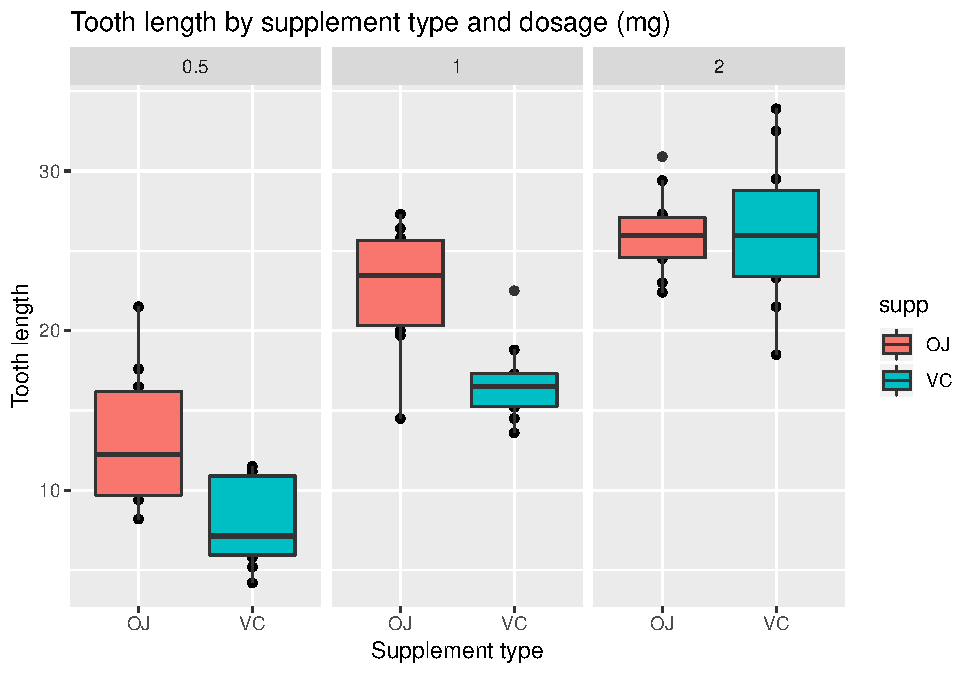
\includegraphics{figures/fig-qplot-1.pdf}

As you can see, the boxes of the supplement types overlap within the
0.5mg dose and the 2mg dose. It appears that the biggest difference in
tooth length appears between the supplement types when given the 1mg
dose. Overall, tooth length was highest in the 2mg dose group,
regardless of supplement type administered.

Since it appears the variances of tooth growth differ by supplement and
possibly by dose, we will need to perform Welch's t-tests for unequal
variances when comparing tooth length by supplement and by dose.

The type of hypothesis testing performed below assumes the following: -
Variables are independent and identically distributed (IID) - Variances
of tooth growth differ by supplement and dose - The distribution of
tooth growth is normal/gaussian

I compared tooth growth (len) by type of vitamin supplement (supp) using
hypothesis test with H0 = no difference in tooth growth by vitamin
supplement.

\begin{Shaded}
\begin{Highlighting}[]
\CommentTok{# Use confidence intervals and/or hypothesis tests to compare tooth growth by supp and dose. }
\CommentTok{# (Only use the techniques from class, even if there's other approaches worth considering)}
        \CommentTok{#Since the variances appear to be unequal, we need a Welch's t-test:}
        \KeywordTok{t.test}\NormalTok{(len }\OperatorTok{~}\StringTok{ }\NormalTok{supp, }\DataTypeTok{paired =} \OtherTok{FALSE}\NormalTok{, }\DataTypeTok{var.equal =} \OtherTok{FALSE}\NormalTok{, }\DataTypeTok{data =}\NormalTok{ ToothGrowth)}
\end{Highlighting}
\end{Shaded}

\begin{verbatim}
## 
##  Welch Two Sample t-test
## 
## data:  len by supp
## t = 1.9153, df = 55.309, p-value = 0.06063
## alternative hypothesis: true difference in means is not equal to 0
## 95 percent confidence interval:
##  -0.1710156  7.5710156
## sample estimates:
## mean in group OJ mean in group VC 
##         20.66333         16.96333
\end{verbatim}

\begin{Shaded}
\begin{Highlighting}[]
\NormalTok{        ttest =}\StringTok{ }\KeywordTok{t.test}\NormalTok{(len }\OperatorTok{~}\StringTok{ }\NormalTok{supp, }\DataTypeTok{paired =} \OtherTok{FALSE}\NormalTok{, }\DataTypeTok{var.equal =} \OtherTok{FALSE}\NormalTok{, }\DataTypeTok{data =}\NormalTok{ ToothGrowth)}
        \KeywordTok{length}\NormalTok{(ttest)}
\end{Highlighting}
\end{Shaded}

\begin{verbatim}
## [1] 9
\end{verbatim}

\begin{Shaded}
\begin{Highlighting}[]
\NormalTok{        pvalue =}\StringTok{ }\KeywordTok{round}\NormalTok{(ttest}\OperatorTok{$}\NormalTok{p.value, }\DecValTok{9}\NormalTok{)}
\end{Highlighting}
\end{Shaded}

Since the p-value associted with this test (0.0606345)
\textgreater{}0.05, we fail to reject the null that average tooth length
is significantly different by supplement type.

However, what if our null hypothesis is that those taking the OJ
supplement will have greater tooth growth than those taking the VC
supplement?

In this test, we specify a one-sided test:

\begin{Shaded}
\begin{Highlighting}[]
\CommentTok{#What about a hypothesis that mean tooth length is greater when given the OJ supplement?}
\NormalTok{        oneside =}\StringTok{ }\KeywordTok{t.test}\NormalTok{(len }\OperatorTok{~}\StringTok{ }\NormalTok{supp, }\DataTypeTok{alternative =} \StringTok{"greater"}\NormalTok{, }\DataTypeTok{paired =} \OtherTok{FALSE}\NormalTok{, }\DataTypeTok{var.equal =} \OtherTok{FALSE}\NormalTok{, }\DataTypeTok{data =}\NormalTok{ ToothGrowth)}
\NormalTok{        pvalueone =}\StringTok{ }\KeywordTok{round}\NormalTok{(oneside}\OperatorTok{$}\NormalTok{p.value, }\DecValTok{9}\NormalTok{)}
\end{Highlighting}
\end{Shaded}

Performing a one-sided test, we find a significant p-value of 0.0303173
\textless{} 0.05, so we reject the null hypothesis that the true
difference in means is not greater than 0. This supports that on
average, those in the OJ supplement group have greater tooth length than
those in the VC supplement group.

Next, I examined whether tooth growth was significantly different by
dose with H0 = no difference in tooth growth by dose. Note - Due to the
project specifications, I will need to produce multiple t-tests instead
of an ANOVA or regression.

\begin{Shaded}
\begin{Highlighting}[]
        \CommentTok{#THe variance for the 0.5 dose looks slightly larger, so use unequal just to be safe}
        \CommentTok{#we first need to compare the 0.5 dose vs. the 1.0 dose, }
        \CommentTok{#then the 1.0 dose vs. the 2.0 dose, then the 0.5 dose vs. 2.0 dose}
        
        \CommentTok{#First, create three subsets so that dose is only two levels:}
        \CommentTok{# using subset function}
\NormalTok{        halfvsone =}\StringTok{ }\KeywordTok{subset}\NormalTok{(ToothGrowth, dose}\OperatorTok{<}\DecValTok{2}\NormalTok{) }
        
\NormalTok{        onevstwo =}\StringTok{ }\KeywordTok{subset}\NormalTok{(ToothGrowth, dose}\OperatorTok{>}\FloatTok{0.5}\NormalTok{)}
        
\NormalTok{        halfvstwo =}\StringTok{ }\KeywordTok{subset}\NormalTok{(ToothGrowth, dose}\OperatorTok{==}\FloatTok{0.5} \OperatorTok{|}\StringTok{ }\NormalTok{dose}\OperatorTok{==}\DecValTok{2}\NormalTok{)}
        
        \CommentTok{#0.5 vs 1 mg:}
\NormalTok{        halfvsonetest =}\StringTok{ }\KeywordTok{t.test}\NormalTok{(len }\OperatorTok{~}\StringTok{ }\NormalTok{dose, }\DataTypeTok{paired =} \OtherTok{FALSE}\NormalTok{, }\DataTypeTok{var.equal =} \OtherTok{FALSE}\NormalTok{, }\DataTypeTok{data =}\NormalTok{ halfvsone)}
\NormalTok{        p.5vs1 =}\StringTok{ }\KeywordTok{round}\NormalTok{(halfvsonetest}\OperatorTok{$}\NormalTok{p.value, }\DecValTok{7}\NormalTok{)}
        
        \CommentTok{#1 vs 2 mg:}
\NormalTok{        onevstwotest =}\StringTok{ }\KeywordTok{t.test}\NormalTok{(len }\OperatorTok{~}\StringTok{ }\NormalTok{dose, }\DataTypeTok{paired =} \OtherTok{FALSE}\NormalTok{, }\DataTypeTok{var.equal =} \OtherTok{FALSE}\NormalTok{, }\DataTypeTok{data =}\NormalTok{ onevstwo)}
\NormalTok{        p1vs2 =}\StringTok{ }\KeywordTok{round}\NormalTok{(onevstwotest}\OperatorTok{$}\NormalTok{p.value, }\DecValTok{5}\NormalTok{)}
        
        \CommentTok{#0.5 vs 2 mg:}
\NormalTok{        halfvstwotest =}\StringTok{ }\KeywordTok{t.test}\NormalTok{(len }\OperatorTok{~}\StringTok{ }\NormalTok{dose, }\DataTypeTok{paired =} \OtherTok{FALSE}\NormalTok{, }\DataTypeTok{var.equal =} \OtherTok{FALSE}\NormalTok{, }\DataTypeTok{data =}\NormalTok{ halfvstwo)}
\NormalTok{        p.5vs2 =}\StringTok{ }\NormalTok{halfvstwotest}\OperatorTok{$}\NormalTok{p.value}
\end{Highlighting}
\end{Shaded}

As you can see by the output in the t-tests, dose level significantly
impacts the average tooth length and we reject the null hypotheses in
all the tests (that dose does not impact tooth length). Those who were
given the 0.5 mg dose had a significantly lower average tooth length
compared to those given the 1.0 mg dose (p = 0.0000001) or those given
the 2.0 mg dose (p \textasciitilde{} 0.0000). Furthermore, those given
the 1.0 mg dose had a significantly lower average tooth length compared
to those given the 2.0 mg dose (p = 0.00002). In sum, higher dose =
greater tooth length.


\end{document}
